\documentclass[letterpaper]{article}
\usepackage[submission]{aaai2027}
\usepackage[hyphens]{url}
\usepackage{graphicx}
\urlstyle{rm}
\def\UrlFont{\rm}
\usepackage{natbib}
\usepackage{caption}
\usepackage{booktabs}
\usepackage{amsmath}
\usepackage{amssymb}
\frenchspacing
\pdfinfo{/TemplateVersion (2027.1)}
\setcounter{secnumdepth}{0}

\title{Learning Role-Aware Submodular Cut Selection for Dual-Source Rotary Cluster-Tool Scheduling}
\author{Anonymous Submission}
\affiliations{}

\begin{document}
\maketitle

\begin{abstract}
We study a rotary semiconductor cluster tool in which product wafers and reusable process-enabling carrier (PEC) wafers enter from different stores and share robots, load locks, and process chambers.
Its four-wafer rotary recipe and pair-exchange recipe couple discrete assignment with continuous-time resource coordination.
We formulate an end-to-end mixed-integer model that includes serial alignment, loaded and empty robot motion, load-lock capacity, PEC reuse, chamber rotation, and cleaning.
At the solver level, standard cut-quality features cannot distinguish candidates with similar efficacy but different mixtures of discrete and continuous support.
Our key observation is that absolute row coefficients, grouped by solver-observable variable roles, provide this missing information without application labels or variable-name parsing.
The same role view also yields a structure-preserving binary-skeleton (SPBS) warm start: a temporary copy fixes high-confidence assignment, activation, cleaning-epoch, and slot decisions, solves only for a consistent incumbent, and passes that incumbent back to the original MIP.
We append ten such features to the thirteen HEM features, predict cut cardinality and order hierarchically, and complete a policy-anchored subset by greedily maximizing a monotone role-coverage objective.
The objective combines cut quality, concave role coverage, and facility-location representativeness, giving the structural layer an explicit approximation guarantee rather than a fixed quota heuristic.
Because SPBS only supplies an incumbent and the cut selector selects only SCIP-generated cuts, neither component changes the feasible set.
Small exact solves validate the formulation and expose a computational cliff on the mixed $8+8$ case; multi-seed selector results are not yet available.
\end{abstract}

\section{Introduction}

A schedule for a semiconductor cluster tool must specify more than a chamber order.
It must decide when each wafer leaves storage, which robot carries it, which load-lock slot it occupies, and when a chamber exposes the required side.
We consider a tool with two material sources: product wafers start at load ports, whereas process-enabling carrier (PEC) wafers start at a separate store and can be reused.
Both flows share an atmospheric robot (ATR), a vacuum robot (VTR), two load locks, and two rotary chambers.
The objective is the return time of the last product wafer.

The equipment combines two recipes whose timing structures are different.
The $4\times1$ recipe fills the two sides of a four-pocket chamber before processing.
The $2\times2$ recipe forms a contiguous exchange chain in which an incoming pair replaces an outgoing pair between consecutive exposures.
Existing cluster-tool studies address cyclic operation, concurrent wafer types, or non-cyclic robot sequencing \cite{ahn2025cluster,kim2025adaptive,li2025cyclic,yang2025residency}.
Our setting adds a finite reusable PEC stream, two rotary recipes, a single-slot aligner, and cleaning batches.
Aggregating any of these operations can create a physically impossible schedule: a pair cannot occupy the aligner together, a robot cannot perform two loaded moves without repositioning, and the same PEC wafer cannot support overlapping chamber jobs.

The detailed formulation is difficult to solve because it couples assignment binaries with a large continuous-time disjunctive schedule.
SCIP strengthens such models by generating cutting planes and retaining a subset at each separation round \cite{bestuzheva2023scip}.
Learned selectors estimate a score for each cut \cite{huang2022learning}, predict both cardinality and order \cite{wang2023hem}, or adapt the weights of SCIP's hybrid score \cite{turner2023adaptive}.
These methods describe efficacy, violation, support, and objective alignment well.
They do not, however, explicitly describe whether a cut is concentrated on binary decisions, continuous auxiliaries, or a coupling between the two.
Consequently, a high-quality prefix can contain several cuts with similar variable support while omitting a different role that is also active in the relaxation.

We address this issue with role-aware hierarchical cut selection.
For every candidate row, we distribute the absolute coefficient mass over variable roles available directly from SCIP; no variable-name parser or application label is used.
These role features augment a HEM-style policy that first chooses how many cuts to retain and then orders the candidates.
Because an ordered neural decoder can still repeat the same structural pattern, we apply a policy-anchored submodular completion layer that balances quality, role coverage, and candidate representativeness.
Figure~\ref{fig:pipeline} shows the complete path from the scheduling MIP to the selected SCIP cuts.

The same structural perspective is also useful before the first separation round.
Large mixed instances can spend substantial time without a feasible incumbent, especially when a cleaning trigger occurs inside a $2\times2$ exchange chain.
We therefore add a structure-preserving binary-skeleton warm start.
It fixes only high-confidence discrete choices in a temporary model copy, including canonical wafer-pair assignments, activation indicators, cleaning epochs, and load-lock slots, while leaving the original MIP unchanged.
The resulting incumbent improves the primal side of the exact solve without excluding any globally optimal solution.

\begin{figure*}[t]
\centering
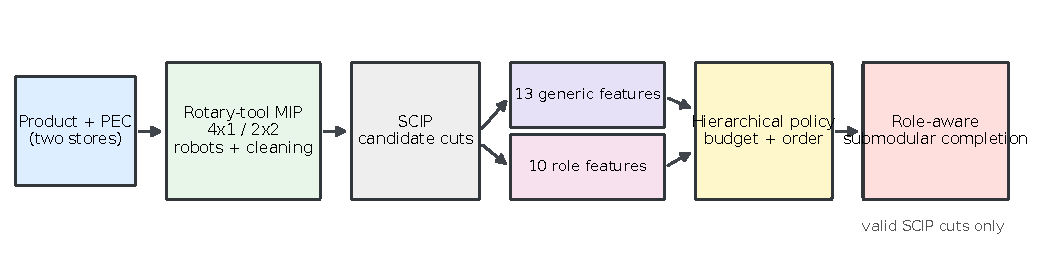
\includegraphics[width=0.96\textwidth]{rdmct_pipeline.pdf}
\caption{Overview. The scheduling model supplies a difficult mixed discrete--continuous instance, but the cut representation itself is domain independent. SCIP produces valid candidate cuts; the learned policy chooses a budget and an order from generic and variable-role features; role-submodular completion balances quality, coverage, and representativeness before returning the selected prefix.}
\label{fig:pipeline}
\end{figure*}

This paper makes four technical contributions.
First, it gives an end-to-end mixed-integer model of dual-source rotary scheduling, including operations that are commonly hidden inside aggregate transfer or chamber durations.
Second, it introduces SPBS, a role-guided initial-solution strategy that converts the scheduling structure into a feasible SCIP incumbent without constraining the original branch-and-bound search.
Third, it introduces a name-invariant cut representation that records how a cut acts on discrete and continuous variable roles and can therefore be computed for arbitrary SCIP models.
Fourth, it combines learned cardinality and ordering with a monotone role-aware submodular objective whose greedy completion has a standard approximation guarantee, while retaining SCIP's cut-validity guarantees.
The empirical study is designed to separate these contributions through a no-warm-start baseline, SPBS ablations, a 13D HEM baseline, a 23D feature-only variant, and the full submodular policy.

\section{Related Work}

\paragraph{Cluster-tool scheduling.}
Cluster-tool schedules have been constructed with cyclic robot rules, Petri nets, mathematical programming, and reinforcement learning.
Recent MIP formulations improve non-cyclic scheduling by representing precedence relations directly \cite{ahn2025cluster}, while learning-based work chooses robot and wafer-release actions without a fixed cyclic sequence \cite{kim2025adaptive}.
Other studies handle concurrent wafer types and residency-time constraints \cite{li2025cyclic,yang2025residency}.
These models motivate explicit robot and module timing, but they do not cover the combination studied here: product and reusable PEC sources, two rotary recipes, and cleaning within one finite-horizon schedule.

\paragraph{Learning inside exact optimization.}
Machine learning has been used to replace or guide expensive decisions in exact solvers.
Examples include branching policies trained across MIP families \cite{limip2023}, reinforcement learning from reconstructed branch-and-bound trajectories \cite{parsonson2023retro}, and learned surrogates inside cutting-plane algorithms \cite{mana2024cutting}.
Scheduling work has likewise combined learned predictions with optimization layers that recover feasibility \cite{kotary2022jsp}.
Our learned component does not construct a schedule or a cut.
It acts only at SCIP's cut-selection interface, leaving the model and the validity of generated inequalities unchanged.

\paragraph{Learning to select cuts.}
Cut selection must balance relaxation improvement against LP and callback overhead.
Huang et al. learn scores for individual cuts \cite{huang2022learning}; HEM treats the retained cardinality and ordered subset as coupled decisions \cite{wang2023hem}; and Adaptive Cut Selection predicts the weights of SCIP's hybrid score \cite{turner2023adaptive}.
The broader design space is reviewed by Deza and Khalil \cite{deza2023survey}.
We retain HEM's separation between cardinality and ordering, but add solver-observable variable roles and a policy-anchored submodular completion layer.
In our comparisons, HEM receives exactly the original 13 generic features; ACS-Tuned is distinguished from full ACS, which requires held-out instance-level weight predictions.

\section{Dual-Source Rotary Scheduling Model}

\paragraph{Material flow.}
Let $W=W^{4\times1}\cup W^{2\times2}$ be the product wafers, $Q$ the reusable PEC tokens, and $C=\{\mathrm{CH2},\mathrm{CH3}\}$ the rotary chambers.
A product wafer follows
\[
\begin{aligned}
\mathrm{LP}&\rightarrow\mathrm{ATR}\rightarrow\mathrm{AL}
\rightarrow\mathrm{LL}^{up}\rightarrow\mathrm{VTR}\\
&\rightarrow\mathrm{CH}\rightarrow\mathrm{LL}^{low}
\rightarrow\mathrm{ATR}\rightarrow\mathrm{LP},
\end{aligned}
\]
whereas a PEC wafer follows
$\mathrm{PECStore}\rightarrow\mathrm{VTR}\rightarrow\mathrm{CH}
\rightarrow\mathrm{VTR}\rightarrow\mathrm{PECStore}$.
Product wafers of the same recipe are paired.
If a recipe contains an odd final wafer, that wafer is paired with one PEC token rather than with a fictitious empty wafer.

\paragraph{Rotary recipes.}
An active $4\times1$ batch assigns one pair to each chamber side.
The chamber executes front load, half rotation, back load, processing, back unload, half rotation, and front unload.
If only one product pair remains, the unused side is filled by a PEC pair; such a filler is allowed only in the tail batch of a chamber sequence.
For $2\times2$, product pairs form a contiguous prefix chain between a PEC head and a PEC tail.
Each product pair appears in two adjacent processing exposures, and the interval between them contains the physical pair exchange.
This construction permits the necessary bridge wait but does not create an ``empty wafer'' decision.

\paragraph{Assignments and time intervals.}
Let $P$ be the product-pair set, $B_c$ the candidate $4\times1$ batches on chamber $c$, and $K_c$ the candidate $2\times2$ positions.
Binary variables $x^F$ and $x^M$ assign each pair exactly once:
\begin{equation}
\sum_{c\in C}\left(
\sum_{b\in B_c}\sum_{h=1}^{2}x^F_{pbhc}
+\sum_{k\in K_c}x^M_{pkc}\right)=1,
\quad p\in P.
\label{eq:assignment}
\end{equation}
Each physical action $a$ has start $s_a$, end $e_a$, and duration $d_a$.
For two optional tasks $a$ and $b$ using the same unary resource, an order variable $y_{ab}$ enforces
\begin{align}
s_b &\ge e_a+\delta_{ab}-M(1-y_{ab}),\\
s_a &\ge e_b+\delta_{ba}-My_{ab},
\label{eq:resource}
\end{align}
where $\delta$ is the endpoint-dependent empty reposition time.
The same construction coordinates ATR, VTR, chamber windows, and load-lock slots.

\paragraph{Physical details that affect feasibility.}
AL has one slot, so the two wafers carried by ATR are calibrated serially: ATR places one wafer, removes it after calibration, and only then places its companion.
ATR and VTR tasks include pickup, loaded travel, placement, and the empty move required before the next pickup.
Upper and lower load locks have two explicit slots.
A PEC job occupies one chamber-bound token from VTR load start through VTR unload end, which prevents overlapping reuse.
After a configurable number of full-chamber processing cycles, cleaning is represented as a pure-PEC rotary batch with the same VTR and chamber-side semantics as production.

\paragraph{Objective.}
The primary objective minimizes the return makespan
\begin{equation}
\min C_{\max},\qquad
C_{\max}\ge C^{\mathrm{return}}_w\quad (w\in W).
\end{equation}
For schedule visualization, an optional second phase fixes $C_{\max}$ and minimizes convex penalties on avoidable waiting in chambers, load locks, and wafer routes.
This phase is lexicographic: it cannot trade a worse makespan for a visually smoother schedule.
It is disabled in the generic cut-selection benchmarks.

\section{Structure-Preserving Binary-Skeleton Warm Start}

Detailed scheduling MIPs often need a useful incumbent before cut selection or branching decisions can be evaluated meaningfully.
However, directly fixing a complete schedule would risk encoding a brittle heuristic path.
SPBS instead fixes a small, interpretable binary skeleton in a temporary model copy and uses SCIP to complete all remaining timing and resource decisions.
The produced solution file is then read by the original model as an incumbent.
No SPBS bound, assignment, or ordering constraint is added to the original solve.

\paragraph{Binary structure matrix.}
For each binary variable $x_j$, SPBS builds a one-hot role vector
\[
z_j\in\{0,1\}^{|\mathcal H|},\qquad
\mathcal H=\{A,U,E,L,R_{\ell},R_h,O\},
\]
where $A$ denotes wafer or batch assignment, $U$ activation indicators, $E$ cleaning or process epochs, $L$ load-lock slot choices, $R_{\ell}$ low-risk local resource orders, $R_h$ high-risk VTR orders, and $O$ timing or residual binaries.
The matrix $Z=[z_j]_j$ is the same kind of structural object as the role-mass cut features: it converts variable-level semantics into a solver-side role summary before a neural or heuristic decision is made.
Unlike the cut features, SPBS may use the scheduling model's own variable taxonomy because it is an instance-construction heuristic rather than a cross-domain cut representation.

\paragraph{Role confidence and fixing policy.}
Each role has a confidence $\kappa_h$ and a fixing rule.
Assignment, activation, cleaning-epoch, and slot variables have high confidence because they follow directly from the recipe grammar.
ATR, aligner, and load-lock local orders are medium-confidence because the canonical flow fixes many nonconflicting precedences.
VTR order is high impact but more fragile, so SPBS first tries a full profile and then falls back to a relaxed profile in which VTR-order binaries remain free.
Formally, for a temporary model $\tilde M$, SPBS fixes
\[
\ell_j=u_j=\hat x_j
\quad\text{only when}\quad
\pi(z_j,\kappa_{h(j)},\mathrm{profile})=\mathrm{fix},
\]
where $\hat x_j$ is the skeleton value and $\pi$ is the role/profile policy.
All continuous start and completion times, waiting variables, and unfixed resource orders are left for SCIP.

\paragraph{PEC-aware cleaning skeleton.}
The skeleton follows the physical recipes.
For $4\times1$, it fills complete four-wafer rotary batches and uses PEC pairs only for a tail side when the product count is odd.
For $2\times2$, product pairs form contiguous exchange chains bounded by PEC head and tail pairs.
When the cleaning interval is reached inside a $2\times2$ chain, SPBS does not require the chamber to finish all remaining product pairs.
Instead, the cycle that triggers cleaning places PEC in the side that will be cleaned next and replaces the remaining in-chamber wafers by PEC before the cleaning batch.
The subsequent segment resumes product exchange after cleaning.
This mirrors the equipment logic that cleaning can start after the trigger cycle has converted the chamber to a pure-PEC state.

\paragraph{Optimality-preserving use.}
SPBS affects only the incumbent pool.
If the temporary model finds a feasible solution, SCIP receives it through the normal solution interface; if it fails, the original solve proceeds without the warm start.
Therefore the original feasible region, valid inequalities, branching decisions available to SCIP, and global optimality proof are unchanged.
The expected benefit is a stronger primal bound, faster time to first incumbent, and better primal-dual integral, not a relaxation of the proof requirement.

\section{Role-Aware Hierarchical Cut Selection}

At separation round $t$, SCIP supplies candidate rows $\mathcal C_t$ and a maximum retained cardinality.
Our selector executes four steps: compute cut features, predict a budget, predict an ordered subset, and complete it under a role-aware submodular objective.
Only the final ordering and retained prefix are returned; cut coefficients and right-hand sides are never modified.

\paragraph{Generic cut features.}
The 13D HEM representation contains objective parallelism, efficacy, support, integral support, normalized violation, four statistics of the cut coefficients, and four statistics of objective coefficients.
These measurements describe immediate cut quality and scaling.
They do not identify which variable types contribute that support.

\paragraph{Variable-role coefficient mass.}
For a candidate cut $i$ with row $\sum_j a_{ij}x_j\le b_i$, let
\[
\mathcal G=\{B,I,C_{\mathrm{obj}},C_{\mathrm{aux}},O\}
\]
denote binary, general-integer, objective-active continuous, continuous auxiliary, and unknown roles.
The role mass is
\begin{equation}
p_{ig}=\frac{\sum_{j:\,x_j\in g}|a_{ij}|}
{\sum_j|a_{ij}|+\epsilon}.
\label{eq:role_mass}
\end{equation}
All role assignments come from SCIP variable metadata.
In particular, no scheduling-specific variable name is inspected.

\begin{table}[t]
\caption{Ten role-aware features appended to the 13 generic features. Each mass is normalized by $\sum_j|a_{ij}|+\epsilon$.}
\label{tab:features}
\centering
\small
\begin{tabular}{lp{0.55\columnwidth}}
\toprule
Count & Features \\
\midrule
5 & Coefficient mass on $B$, $I$, $C_{\mathrm{obj}}$, $C_{\mathrm{aux}}$, and $O$ \\
1 & Mass on variables with finite global lower and upper bounds \\
1 & Positive-coefficient mass \\
1 & Disc.--cont. coupling $4(p_{iB}+p_{iI})(p_{iC_{\mathrm{obj}}}+p_{iC_{\mathrm{aux}}})$ \\
1 & Largest non-residual role mass \\
1 & Role entropy $-\sum_g p_{ig}\log p_{ig}/\log|\mathcal G|$ \\
\bottomrule
\end{tabular}
\end{table}

Table~\ref{tab:features} lists the remaining row-geometry features.
The coupling term is zero when a cut acts only on one side of the discrete--continuous split and is largest for balanced support.
The dominant mass and entropy distinguish a focused cut from one that mixes many roles.
The complete candidate vector has 23 dimensions and is invariant to variable renaming.

\paragraph{Budget and ordered subset.}
A high-level policy maps the candidate feature set to a retained fraction $\rho_t$, which is clipped by SCIP's limit and an implementation cap to obtain $k_t$.
A pointer network then samples or greedily decodes an ordered sequence of candidates.
Training minimizes the observed primal-dual integral through REINFORCE updates with an exponential moving-average baseline.
Independent SCIP processes collect complete rollouts, and their trajectories are aggregated before each parameter update.
We therefore refer to the implementation as parallel hierarchical policy-gradient training: environment rollouts are parallel, whereas parameter updates are centralized.

\paragraph{Policy-anchored role-submodular completion.}
The neural order may devote most of its budget to one structural pattern.
We retain its first $\lceil\gamma k_t\rceil$ candidates as anchors $A_t$ and form an expansion pool $R_t$ of at most $\alpha k_t$ candidates by appending rows with high normalized structural quality $q_i$.
For $S\subseteq R_t$, define
\begin{align}
F_t(S)={}&\sum_{i\in S}(.35q_i+.20r_i)
+ .25\sum_{g\in\mathcal G}d_g
\sqrt{\sum_{i\in S}p_{ig}}\nonumber\\
&+\frac{.20}{|R_t|}\sum_{u\in R_t}\max_{i\in S}s_{ui},
\label{eq:submodular}
\end{align}
where $r_i$ is the normalized neural rank prior, $d_g$ is role demand in $R_t$, and $s_{ui}\in[0,1]$ is the clipped cosine similarity between generic--role cut descriptors.
The first term preserves immediate quality and the learned order.
The concave second term gives diminishing returns to repeated role mass, while the facility-location term rewards a subset that represents the candidate pool without an explicit pairwise penalty.

Starting from $A_t$, we repeatedly add the candidate with largest marginal gain $F_t(S\cup\{i\})-F_t(S)$ until $|S|=k_t$.
All coefficients in Eq.~\eqref{eq:submodular} are nonnegative; hence its modular, concave-over-modular, and facility-location components are monotone submodular.
For fixed anchors, the residual objective $F_t(A_t\cup T)-F_t(A_t)$ remains normalized, monotone, and submodular over $R_t\setminus A_t$.
Cardinality-constrained greedy therefore obtains at least a $(1-1/e)$ fraction of the best residual gain achievable inside $R_t$ \cite{nemhauser1978submodular}.
We use $\alpha=2$ and $\gamma=.25$, selected on validation and fixed for every family.
The layer only chooses among SCIP-generated valid cuts and therefore cannot remove any integer-feasible solution.

\section{Experimental Protocol}

The experiments test three claims separately.
First, role features should improve cut selection over a 13D policy under the same training and solver budgets.
Second, submodular completion should add value beyond the features alone.
Third, a name-invariant representation should remain usable outside the scheduling formulation, although transfer gains are not assumed.

\paragraph{Data.}
The scheduling generator uses disjoint size and recipe-ratio splits.
Training contains pure and mixed instances with at most 12 product wafers; validation contains 16-wafer instances; test contains 24--32 wafers and recipe ratios not seen in training.
For cross-family tests, we generate set cover, multidimensional knapsack, capacitated facility location, and maximum-weight independent set instances at three scales.
MIPLIB 2017 provides a heterogeneous external set \cite{gleixner2021miplib}.

\paragraph{Baselines and ablations.}
We compare SCIP Default, ACS-Tuned, full ACS when held-out instance predictions are available, HEM with a separately trained 13D checkpoint, and the proposed 23D policy.
HEM and our policy use identical instances, optimizer budgets, candidate caps, and random seeds.
For initial solutions, we compare no warm start, the full SPBS profile, and the relaxed SPBS profile that leaves VTR-order binaries unfixed.
The warm-start ablation is crossed with SCIP Default and the learned cut selectors to separate primal-incumbent effects from separation-policy effects.
The cut-selection ablation adds the 10 role features while disabling submodular completion; the full model then enables Eq.~\eqref{eq:submodular}.
Additional ablations vary candidate cap, retained cardinality, greedy versus beam decoding, expansion factor $\alpha$, anchor ratio $\gamma$, each submodular component, and the SPBS role-fixing policy.

\paragraph{Metrics and statistics.}
The primary anytime metric is primal-dual integral (PDI).
We also record shifted geometric mean runtime, final gap, node count, time to first incumbent, incumbent acceptance rate, optimality rate, warm-start construction time, feature-extraction time, and neural inference time.
Scheduling runs additionally report makespan and robot/chamber utilization.
All comparisons are paired by instance and SCIP seed.
The formal study uses five training seeds and at least ten SCIP seeds, with bootstrap 95\% confidence intervals, paired Wilcoxon tests, and Holm correction across families.

\paragraph{Implementation.}
Experiments use Python 3.13.5, PySCIPOpt 6.1.0, NumPy 2.1.3, and PyTorch 2.11.0.
Candidate pools are capped at 128 and retained prefixes at 16 unless chosen otherwise on validation.
The pointer network has a 128-dimensional hidden state and one glimpse.
The 13D and 23D checkpoints are trained separately; a schema tag prevents legacy 23D weights from being loaded after the feature semantics changed.

\section{Current Validation}

\paragraph{Formulation checks.}
Table~\ref{tab:preliminary} summarizes deterministic validation runs with two chambers, 110-second $4\times1$ processing, 50-second $2\times2$ exposures, and reusable PEC tokens.
These runs test model connectivity and the expected computational regime; they do not compare learned selectors.

\begin{table}[t]
\caption{Recorded formulation-validation runs. The mixed $8+8$ instance has an incumbent at the 60-second limit but retains a large gap.}
\label{tab:preliminary}
\centering
\small
\begin{tabular}{lrrrr}
\toprule
Instance & Vars & Cons. & $C_{\max}$ & Status \\
\midrule
Pure $4\times1$ (4) & 684 & 1,645 & 388 & optimal \\
Pure $2\times2$ (4) & 876 & 1,959 & 324 & optimal \\
Mixed (4+4) & 1,182 & 2,765 & 508 & optimal \\
Mixed (8+8) & 2,932 & 7,995 & 1,150 & limit \\
\bottomrule
\end{tabular}
\end{table}

The two pure four-wafer instances solve at the root in under one second.
The mixed $4+4$ instance requires 797 nodes and about 11 seconds.
The mixed $8+8$ instance explores 7,779 nodes in 60 seconds and ends with a 99.98\% relative gap.
The change is not evidence that a learned selector will succeed, but it identifies the mixed regime in which cut management can be measured.

\paragraph{SPBS interface check.}
We also tested the warm-start interface on a larger mixed cleaning instance with 53 $4\times1$ wafers, 43 $2\times2$ wafers, two chambers, ten candidate batches, thirteen planning steps, eight PEC tokens, and a cleaning interval of ten full-chamber process cycles.
This is the regime in which a naive ``finish the whole $2\times2$ chain before cleaning'' rule is infeasible: 43 wafers form 22 product pairs, but cleaning must be allowed to interrupt the chain after the trigger cycle has converted the chamber to PEC.
The SPBS generator splits the $2\times2$ chain into PEC-bounded segments, solves a temporary fixed-skeleton copy, and writes a SCIP solution with makespan 7,086 seconds.
Reading that solution into the unfixed original LP returns a feasible solution certificate and stores it as an incumbent before branch-and-bound starts.
This check validates the incumbent pathway and the PEC-aware cleaning logic; it is not counted as evidence for the final learned-selector comparison.

\paragraph{Status of learned-policy results.}
The HEM training is still running, and the 23D policy must be retrained because the postprocessor used during its rollout transition changed from fixed quota repair to Eq.~\eqref{eq:submodular}.
Accordingly, this draft makes no claim of improvement over SCIP, ACS, or HEM.
The final submission must replace this paragraph with frozen paired results, the feature-only and submodular ablations, cross-scale tests, cross-family tests, and callback-overhead measurements.

\section{Limitations}

The five cut-selection roles are intentionally coarse.
They do not encode constraint-graph topology, indicator semantics, symmetry, or cut provenance.
SPBS uses a more scheduling-specific binary taxonomy and is therefore not a domain-independent warm-start method.
Moreover, SPBS supplies an incumbent rather than a proof shortcut: if the skeleton is poor, SCIP can ignore or improve it, but global optimality still depends on the exact search.
The submodular component weights, expansion factor, and anchor ratio are fixed globally and require validation-only sensitivity analysis before they can be treated as robust defaults.
The scheduling instances use engineering parameters rather than production traces, and the formulation-validation table predates the final multi-seed cut study.
Finally, policy updates are synchronized after rollout collection; asynchronous optimization is outside the present implementation.

\section{Conclusion}

This work connects a detailed dual-source rotary scheduling model with a solver-level learning problem.
The scheduling formulation makes alignment, robot repositioning, load-lock capacity, PEC reuse, rotary exchange, and cleaning explicit.
SPBS first converts high-confidence recipe structure into an incumbent while leaving the original MIP unchanged.
The cut selector then describes each SCIP candidate by generic quality and name-invariant variable-role mass, predicts a cardinality and order, and performs policy-anchored submodular completion without changing any inequality.
The present evidence validates the formulation and the implementation interfaces.
Performance conclusions depend on the frozen multi-seed comparison now in progress.

\bibliography{rdmct_aaai27}
\end{document}
